% This file was created by matlab2tikz.
%
\definecolor{mycolor1}{rgb}{0.00000,0.44700,0.74100}%
\definecolor{mycolor2}{rgb}{0.85000,0.32500,0.09800}%
\definecolor{mycolor3}{rgb}{0.92900,0.69400,0.12500}%
\definecolor{mycolor4}{rgb}{0.49400,0.18400,0.55600}%
%
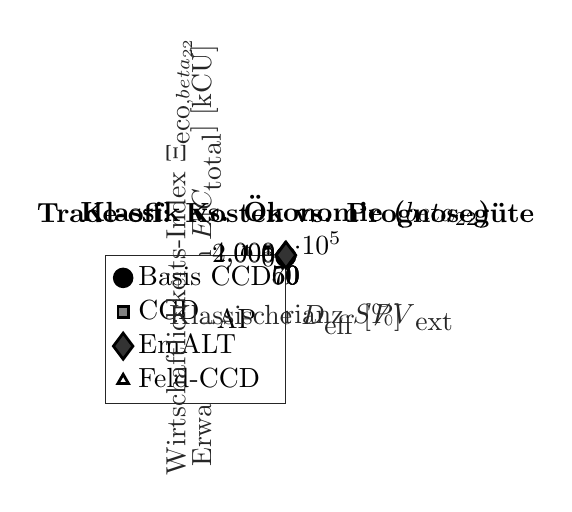
\begin{tikzpicture}

\begin{axis}[%
width=0.422\figurewidth,
height=0.932\figureheight,
at={(0\figurewidth,0\figureheight)},
scale only axis,
xmin=0.00,
xmax=32.53,
xlabel style={font=\color{white!15!black}},
xlabel={Prädiktionsvarianz $\sym{SPV}_{\textnormal{ext}}$},
ymin=0.00,
ymax=144151.22,
ylabel style={font=\color{white!15!black}},
ylabel={Erwartungskosten $\mathbb{E}[\sym{C}_{\textnormal{total}}]$ [kCU]},
axis background/.style={fill=white},
title style={font=\bfseries},
title={\textbf{Trade-off: Kosten vs. Prognosegüte}},
xmajorgrids,
ymajorgrids,
grid style={dotted, opacity=0.25},
legend style={legend cell align=left, align=left, draw=white!15!black}
]
\addplot [color=mycolor1, line width=1.0pt, only marks, mark size=3.2pt, mark=*, mark options={solid, fill=black, draw=black}]
  table[row sep=crcr]{%
30.02	54162.41\\
};
\addlegendentry{Basis \ac{CCD}}

\addplot [color=mycolor2, line width=1.0pt, only marks, mark size=1.9pt, mark=square*, mark options={solid, fill=gray, draw=black}]
  table[row sep=crcr]{%
30.12	48179.27\\
};
\addlegendentry{$\textnormal{\ac{CCD}}_{-\textnormal{\ac{AP}}}$}

\addplot [color=mycolor3, line width=1.0pt, only marks, mark size=4.7pt, mark=diamond*, mark options={solid, fill=white!20!black, draw=black}]
  table[row sep=crcr]{%
2.39	80978.91\\
};
\addlegendentry{\ac{EmALT}}

\addplot [color=mycolor4, line width=1.0pt, only marks, mark size=2.2pt, mark=triangle*, mark options={solid, fill=white, draw=black}]
  table[row sep=crcr]{%
2.60	128706.45\\
};
\addlegendentry{Feld-\ac{CCD}}

\end{axis}

\begin{axis}[%
width=0.422\figurewidth,
height=0.932\figureheight,
at={(0.578\figurewidth,0\figureheight)},
scale only axis,
xmin=46.40,
xmax=72.89,
xlabel style={font=\color{white!15!black}},
xlabel={Klassische $\sym{D}_{\textnormal{eff}}$ [\%]},
ymin=0.00,
ymax=4722.17,
ylabel style={font=\color{white!15!black}},
ylabel={Wirtschaftlichkeits-Index $\Xi_{\textnormal{eco}, \sym{beta}_{22}}$},
axis background/.style={fill=white},
title style={font=\bfseries},
title={\textbf{Klassik vs. Ökonomie ($\sym{beta}_{22}$)}},
xmajorgrids,
ymajorgrids,
grid style={dotted, opacity=0.25}
]
\addplot [color=mycolor1, line width=1.0pt, only marks, mark size=3.2pt, mark=*, mark options={solid, fill=black, draw=black}, forget plot]
  table[row sep=crcr]{%
56.90	606.49\\
};
\node[below, align=center, inner sep=0]
at (axis cs:56.902,838.727) {Basis \ac{CCD}};
\addplot [color=mycolor2, line width=1.0pt, only marks, mark size=1.9pt, mark=square*, mark options={solid, fill=gray, draw=black}, forget plot]
  table[row sep=crcr]{%
50.40	647.18\\
};
\node[below, align=center, inner sep=0]
at (axis cs:50.397,879.417) {$\textnormal{\ac{CCD}}_{-\textnormal{\ac{AP}}}$};
\addplot [color=mycolor3, line width=1.0pt, only marks, mark size=4.7pt, mark=diamond*, mark options={solid, fill=white!20!black, draw=black}, forget plot]
  table[row sep=crcr]{%
68.89	3870.63\\
};
\node[below, align=center, inner sep=0]
at (axis cs:68.888,4102.865) {\ac{EmALT}};
\end{axis}
\end{tikzpicture}%